\setAuthor{Tundmatu autor}
\setRound{lahtine}
\setYear{2009}
\setNumber{G 2}
\setDifficulty{2}
\setTopic{Geomeetriline optika}

\prob{Lääts}
Lääts tekitab esemest $d = \SI{24}{cm}$ kaugusele ekraanile kujutise, mis on esemest \num{3} korda suurem. Leidke läätse fookuskaugus.

\hint
Tasub teha selge joonis ning kasutada sarnaseid kolmnurki.

\solu
Kuna kujutis tekib ekraanile, siis on kujutis tegelik ning tegemist on koondava läätsega.

\begin{center}
	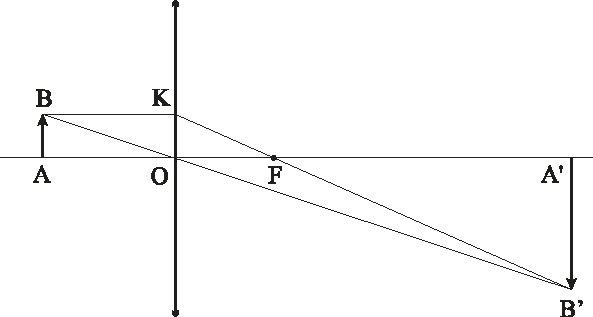
\includegraphics[width=0.9\linewidth]{2009-lahg-02-lah}
\end{center}

Olgu $a$ kaugus esemest läätseni, $k$ kaugus kujutisest läätseni ning $f$ läätse fookuskaugus. Et kujutis on esemest \num{3} korda suurem, siis sarnastest kolmnurkadest $ABO$ ja $A'B'O$
\[
\frac{k}{a}=3 \quad \Rightarrow \quad k=3 a.
\]
Kujutis tekib kugusele $d = \SI{24}{cm}$, seega
\[
a+k=4 a=\SI{24}{cm} \quad \Rightarrow \quad a=\SI{6}{cm}, k=\SI{18}{cm}.
\]
Nüüd läätse valemist
\[
\frac{1}{a}+\frac{1}{k}=\frac{1}{f}
\]
leiame, et $f = \SI{4,5}{cm}$.

\emph{Märkus}. Läätse valemi asemel võib fookuskauguse leidmiseks kasutada sarnaseid kolmnurki $A'B'F$ ja $OKF$. Saame
\[
\frac{k-f}{f}=3 \quad \Rightarrow \quad f=\frac{k}{4}=\SI{4,5}{cm}.
\]
\probend